% informe_r3.tex: cuerpo del informe cuando el diseño descrito es R3 (C1 en los cuatro hilos).
%
% Grupo: Nicolás Araneda, Vicente Calderón y Santiago Muñoz.
% Arquitectura de Computadores, Universidad de los Andes, 2026-2.
%
% Lo incluye informe.tex bajo \ifpeldanotres (make informe PELDANO_INFORME=r3). Ninguna cifra de
% C1 ni de R3 se escribe a mano: vienen de generado/cifras_c1.tex, que rehace tools/report_c1.py
% y que trae al lado de cada una su archivo de origen.
% Generado por tools/report_c1.py (make informe PELDANO_INFORME=r3). No editar a mano.
\newcommand{\ctresAjenasDifNdBandaTreinta}{$+$2{,}1 (0{,}4)}% docs/mediciones/c1/v5_finalistas.txt (copia del registro de la rama minutos-reales, commit 17d7284)
\newcommand{\ctresAjenasGana}{81{,}9}% docs/mediciones/c1/v5_finalistas.txt (copia del registro de la rama minutos-reales, commit 17d7284)
\newcommand{\ctresAjenasGanaBanda}{45{,}5}% docs/mediciones/c1/v5_finalistas.txt (copia del registro de la rama minutos-reales, commit 17d7284)
\newcommand{\ctresAjenasNd}{83{,}0}% docs/mediciones/c1/v5_finalistas.txt (copia del registro de la rama minutos-reales, commit 17d7284)
\newcommand{\ctresAjenasNdBanda}{87{,}9}% docs/mediciones/c1/v5_finalistas.txt (copia del registro de la rama minutos-reales, commit 17d7284)
\newcommand{\ctresAjenasNdBandaTreinta}{90{,}0}% docs/mediciones/c1/v5_finalistas.txt (copia del registro de la rama minutos-reales, commit 17d7284)
\newcommand{\ctresAjenasVentanas}{12\,000}% docs/mediciones/c1/v5_finalistas.txt (copia del registro de la rama minutos-reales, commit 17d7284)
\newcommand{\ctresAmdBandaOrdenes}{8}% docs/mediciones/c1/series_reales.txt
\newcommand{\ctresAmdBandaW}{26\,470}% docs/mediciones/c1/series_reales.txt
\newcommand{\ctresAmdOrdenes}{11}% docs/mediciones/c1/series_reales.txt
\newcommand{\ctresAmdW}{27\,199}% docs/mediciones/c1/series_reales.txt
\newcommand{\ctresAmdahlBarrelMed}{0{,}521}% docs/mediciones/p7/cotas/amdahl.txt
\newcommand{\ctresAmdahlBarrelPred}{0{,}521}% docs/mediciones/p7/cotas/amdahl.txt
\newcommand{\ctresAmdahlF}{29{,}2}% docs/mediciones/c1/ops_roofline.txt
\newcommand{\ctresAmdahlRespMin}{375}% docs/mediciones/c1/ops_roofline.txt
\newcommand{\ctresAmdahlSmax}{1{,}41}% docs/mediciones/c1/ops_roofline.txt
\newcommand{\ctresApagadaCorridas}{46}% docs/mediciones/c1/puerta_a.txt
\newcommand{\ctresApagadaPeor}{203}% docs/mediciones/c1/puerta_a.txt
\newcommand{\ctresApagadaTicks}{920\,000}% docs/mediciones/c1/puerta_a.txt
\newcommand{\ctresApuestaAcciones}{22}% docs/mediciones/c1/series_reales.txt
\newcommand{\ctresApuestaPrecio}{222}% docs/mediciones/c1/series_reales.txt
\newcommand{\ctresApuestaTick}{8\,234}% docs/mediciones/c1/series_reales.txt
\newcommand{\ctresBram}{14}% docs/mediciones/c1/timing.txt
\newcommand{\ctresCeldas}{1\,038}% docs/mediciones/c1/timing.txt
\newcommand{\ctresCeldasRdosMismaSintesis}{1\,015}% docs/mediciones/fondo/r2/timing.txt
\newcommand{\ctresCeldasSobreRdos}{23}% docs/mediciones/c1/timing.txt y fondo/r2/timing.txt
\newcommand{\ctresContDiferencias}{0}% docs/mediciones/c1/contabilidad.txt
\newcommand{\ctresContParciales}{858}% docs/mediciones/c1/contabilidad.txt
\newcommand{\ctresContRtl}{28 de 28}% docs/mediciones/c1/contabilidad_rtl.txt
\newcommand{\ctresContSeries}{3\,052}% docs/mediciones/c1/contabilidad.txt
\newcommand{\ctresDegradacion}{26 de 26}% docs/mediciones/c1/degradacion.txt
\newcommand{\ctresEjecutarCiclos}{154{,}7}% docs/mediciones/c1/ops_roofline.txt
\newcommand{\ctresEjecutarIc}{38{,}7}% docs/mediciones/c1/ops_roofline.txt
\newcommand{\ctresEsperaHiloCero}{291}% docs/mediciones/c1/ops_roofline.txt
\newcommand{\ctresExamenCandadoCasoS}{50{,}6}% docs/mediciones/c1/c1_examen.txt (copia del registro de la rama minutos-reales, commit 17d7284)
\newcommand{\ctresExamenDebajoClon}{16{,}6}% docs/mediciones/c1/c1_examen.txt (copia del registro de la rama minutos-reales, commit 17d7284)
\newcommand{\ctresExamenDifGana}{$+$36{,}1 (2{,}4)}% docs/mediciones/c1/c1_examen.txt (copia del registro de la rama minutos-reales, commit 17d7284)
\newcommand{\ctresExamenDifNd}{$-$7{,}1 (2{,}5)}% docs/mediciones/c1/c1_examen.txt (copia del registro de la rama minutos-reales, commit 17d7284)
\newcommand{\ctresExamenDifNdCasoB}{$+$6{,}3 (2{,}3)}% docs/mediciones/c1/c1_examen.txt (copia del registro de la rama minutos-reales, commit 17d7284)
\newcommand{\ctresExamenDifNdCasoS}{$-$18{,}1 (3{,}1)}% docs/mediciones/c1/c1_examen.txt (copia del registro de la rama minutos-reales, commit 17d7284)
\newcommand{\ctresExamenDifRonda}{$+$152 (52)}% docs/mediciones/c1/c1_examen.txt (copia del registro de la rama minutos-reales, commit 17d7284)
\newcommand{\ctresExamenGana}{81{,}8}% docs/mediciones/c1/c1_examen.txt (copia del registro de la rama minutos-reales, commit 17d7284)
\newcommand{\ctresExamenGanaBanda}{45{,}7}% docs/mediciones/c1/c1_examen.txt (copia del registro de la rama minutos-reales, commit 17d7284)
\newcommand{\ctresExamenNd}{83{,}3}% docs/mediciones/c1/c1_examen.txt (copia del registro de la rama minutos-reales, commit 17d7284)
\newcommand{\ctresExamenNdBanda}{90{,}4}% docs/mediciones/c1/c1_examen.txt (copia del registro de la rama minutos-reales, commit 17d7284)
\newcommand{\ctresExamenRondaCasoB}{$+$431 (62)}% docs/mediciones/c1/c1_examen.txt (copia del registro de la rama minutos-reales, commit 17d7284)
\newcommand{\ctresExamenRondaCasoS}{$-$44 (55)}% docs/mediciones/c1/c1_examen.txt (copia del registro de la rama minutos-reales, commit 17d7284)
\newcommand{\ctresExamenSinRecuperarCasoS}{49{,}4}% docs/mediciones/c1/c1_examen.txt (copia del registro de la rama minutos-reales, commit 17d7284)
\newcommand{\ctresExamenSinRecuperarD}{316}% docs/mediciones/c1/c1_examen.txt (copia del registro de la rama minutos-reales, commit 17d7284)
\newcommand{\ctresExamenVentanas}{3\,600}% docs/mediciones/c1/c1_examen.txt (copia del registro de la rama minutos-reales, commit 17d7284)
\newcommand{\ctresFmin}{48{,}41}% docs/mediciones/c1/timing.txt
\newcommand{\ctresGemeloReales}{203}% docs/mediciones/c1/puerta_b.txt
\newcommand{\ctresHitoDecProm}{530}% docs/mediciones/c1/ticks.txt (por el RTL)
\newcommand{\ctresHitoPolProm}{496}% docs/mediciones/c1/ticks.txt (por el RTL)
\newcommand{\ctresHitoPub}{35}% docs/mediciones/c1/ticks.txt (por el RTL)
\newcommand{\ctresHitoRegProm}{130}% docs/mediciones/c1/ticks.txt (por el RTL)
\newcommand{\ctresHitoTabProm}{271}% docs/mediciones/c1/ticks.txt (por el RTL)
\newcommand{\ctresIcHiloTresMax}{218}% docs/mediciones/c1/ticks.txt (por el RTL)
\newcommand{\ctresIcSumaProm}{466}% docs/mediciones/c1/ticks.txt (por el RTL)
\newcommand{\ctresIntegracionLocal}{27 de 27}% docs/mediciones/ci_local_c1.txt
\newcommand{\ctresIntensidad}{0{,}39}% docs/mediciones/c1/ops_roofline.txt
\newcommand{\ctresKernelCiclos}{530{,}9}% docs/mediciones/c1/ops_roofline.txt
\newcommand{\ctresLimiteGrupo}{1\,131}% docs/puertas.md, criterio 4: la mitad del presupuesto de la ronda 3
\newcommand{\ctresMops}{6{,}89}% docs/mediciones/c1/ops_roofline.txt
\newcommand{\ctresMopsRceroPorClase}{10{,}50}% docs/mediciones/c1/ops_roofline.txt
\newcommand{\ctresMopsRdosPorClase}{3{,}12}% docs/mediciones/c1/ops_roofline.txt
\newcommand{\ctresMopsSobreRdos}{2{,}2}% docs/mediciones/c1/ops_roofline.txt
\newcommand{\ctresOficialPeor}{759}% docs/mediciones/c1/oficial.txt
\newcommand{\ctresOps}{146{,}4}% docs/mediciones/c1/ops_roofline.txt
\newcommand{\ctresOpsBandaPorClase}{21}% docs/mediciones/c1/ops_roofline.txt
\newcommand{\ctresPalabras}{482}% docs/mediciones/c1/tamano.txt
\newcommand{\ctresPalabrasCodigo}{444}% docs/mediciones/c1/tamano.txt
\newcommand{\ctresPalabrasDatos}{38}% docs/mediciones/c1/tamano.txt
\newcommand{\ctresPeorColgado}{916}% docs/mediciones/c1/fases.txt
\newcommand{\ctresPeorFases}{779}% docs/mediciones/c1/fases.txt
\newcommand{\ctresPeorPuertas}{807}% docs/mediciones/c1/puerta_b.txt
\newcommand{\ctresPracticaBandaOrdenes}{4}% ref/c1/c1.py sobre data/practica_meta.csv; docs/mediciones/c1/series_reales.txt
\newcommand{\ctresPracticaBandaPerdida}{3\,168}% ref/c1/c1.py sobre data/practica_meta.csv; docs/mediciones/c1/series_reales.txt
\newcommand{\ctresPracticaBandaW}{21\,392}% ref/c1/c1.py sobre data/practica_meta.csv; docs/mediciones/c1/series_reales.txt
\newcommand{\ctresPracticaCymPerdida}{9\,300}% ref/c1/c1.py sobre data/practica_meta.csv; docs/mediciones/c1/series_reales.txt
\newcommand{\ctresPracticaCymW}{9\,695}% ref/c1/c1.py sobre data/practica_meta.csv; docs/mediciones/c1/series_reales.txt
\newcommand{\ctresPracticaOrdenes}{6}% ref/c1/c1.py sobre data/practica_meta.csv; docs/mediciones/c1/series_reales.txt
\newcommand{\ctresPracticaPerdida}{3\,360}% ref/c1/c1.py sobre data/practica_meta.csv; docs/mediciones/c1/series_reales.txt
\newcommand{\ctresPracticaW}{22\,682}% ref/c1/c1.py sobre data/practica_meta.csv; docs/mediciones/c1/series_reales.txt
\newcommand{\ctresPresupuesto}{2\,262}% tb/tb_proyecto_4.sv: (100000 ns - 9500 ns) / 40 ns
\newcommand{\ctresPuertaBTicks}{4{,}14}% docs/mediciones/c1/puerta_b.txt
\newcommand{\ctresPuertaBVentanas}{200}% docs/mediciones/c1/puerta_b.txt
\newcommand{\ctresRceroMops}{5{,}50}% docs/mediciones/p7/cotas/variantes.csv
\newcommand{\ctresRceroRespPeor}{60}% docs/mediciones/p7/cotas/variantes.csv
\newcommand{\ctresRceroRespProm}{56{,}5}% docs/mediciones/p7/cotas/variantes.csv
\newcommand{\ctresRdosCeldas}{1\,045}% docs/mediciones/p7/cotas/variantes.csv
\newcommand{\ctresRdosMops}{1{,}64}% docs/mediciones/p7/cotas/variantes.csv
\newcommand{\ctresRdosRespMin}{119}% docs/mediciones/fondo/r2/ticks.txt
\newcommand{\ctresRdosRespPeor}{127}% docs/mediciones/p7/cotas/variantes.csv
\newcommand{\ctresRespMin}{399}% docs/mediciones/c1/ticks.txt (por el RTL)
\newcommand{\ctresRespPeor}{783}% gemelo digital, serie de practica a 0,1 ms; igual al RTL de docs/mediciones/c1/ticks.txt
\newcommand{\ctresRespPeorUs}{31{,}3}% gemelo digital, serie de practica a 0,1 ms; igual al RTL de docs/mediciones/c1/ticks.txt
\newcommand{\ctresRespProm}{529{,}9}% gemelo digital, serie de practica a 0,1 ms; igual al RTL de docs/mediciones/c1/ticks.txt
\newcommand{\ctresRespPromUs}{21{,}2}% gemelo digital, serie de practica a 0,1 ms; igual al RTL de docs/mediciones/c1/ticks.txt
\newcommand{\ctresSegMops}{10{,}58}% docs/mediciones/p7/cotas/variantes.csv
\newcommand{\ctresSegRespPeor}{28}% docs/mediciones/p7/cotas/variantes.csv
\newcommand{\ctresSemillas}{10 de 10}% docs/mediciones/c1/timing.txt
\newcommand{\ctresSinteticasGemelo}{1\,081}% docs/mediciones/c1/series.txt
\newcommand{\ctresSinteticasRtl}{1\,050}% docs/mediciones/c1/series.txt
\newcommand{\ctresTablaCeldas}{320}% ref/c1/tablas.py
\newcommand{\ctresTablaUsadas}{348}% ref/c1/tablas.py (USADAS)
\newcommand{\ctresTeslaBandaOrdenes}{4}% docs/mediciones/c1/series_reales.txt
\newcommand{\ctresTeslaBandaW}{20\,795}% docs/mediciones/c1/series_reales.txt
\newcommand{\ctresTeslaOrdenes}{8}% docs/mediciones/c1/series_reales.txt
\newcommand{\ctresTeslaW}{21\,224}% docs/mediciones/c1/series_reales.txt
\newcommand{\ctresTrabajoSerie}{369}% docs/mediciones/c1/ops_roofline.txt
\newcommand{\ctresTrabajoSerieCiclos}{1\,477}% docs/mediciones/c1/ops_roofline.txt
\newcommand{\ctresUsoPresupuesto}{34{,}6}% gemelo digital, serie de practica a 0,1 ms; igual al RTL de docs/mediciones/c1/ticks.txt
\newcommand{\ctresUsoPresupuestoProm}{23{,}4}% gemelo digital, serie de practica a 0,1 ms; igual al RTL de docs/mediciones/c1/ticks.txt


\noindent Diseño que compite: \textbf{R3}, el Espino barrel de cuatro hilos con una tabla de solo lectura de 512 palabras, corriendo \arch{sw/c1.s}. El programa ejecuta el algoritmo C1: la regla de cotas con banda 40 más un desempate, que consiste en una apuesta antes de ver los extremos, una política calculada con un modelo de paseo aleatorio y un candado sobre un rival emulado. La banda 40 sola es la base de C1 y su respaldo, y corre en R0, R1 y R2, los peldaños anteriores de la escalera de co-diseño. Cada número se regenera con \texttt{make informe PELDANO\_INFORME=r3} desde el repositorio (commit \texttt{\commitinforme}), y cada tabla indica su archivo de medición.

% ==============================================================================
\section{Algoritmo de predicción y decisión (3.1)}

\subsection{La información que deja la normalización}

Cada ronda llega normalizada por separado: su precio mínimo es exactamente \cifraPrecioMin{} y su máximo exactamente \cifraPrecioMax{} (\arch{docs/cotas.md}, sección 1). Ver uno de los extremos garantiza entonces que el otro va a llegar antes de que termine la ronda. Comprar en \cifraPrecioMin{} no puede salir peor que comprar en otro tick, y vender en \cifraPrecioMax{} no puede salir peor que vender en otro. La regla 4 del enunciado se cumple: es el formato de la serie, igual para todos los grupos, el programa no guarda ninguna serie y decide el procesador con el precio que recibe.

Según lo que ya se vio, una ronda está en una de cuatro fases: A, ningún extremo; B, solo el \cifraPrecioMax; C, solo el \cifraPrecioMin; D, los dos. La regla base, de cotas con banda 40 (\arch{ref/cotas.py}), compra al ver \cifraPrecioMin{} y vende al ver \cifraPrecioMax. En la fase D ya no queda ningún extremo garantizado por delante, y ahí compra con $p \le 140$ y vende con $p \ge 215$. La banda de 40 unidades se eligió dentro de una meseta: en la población simulada, cualquier banda entre 40 y 76 queda a menos del 2\,\% de la mejor (\arch{docs/cotas.md}, sección 5.2). En la fase A la banda 40 no opera.

\subsection{Un problema limitado por información}

La banda 40 usa casi toda la información que da la normalización, y un rival que llegue a la misma regla termina con el mismo patrimonio. Se midió con torneos de tres rondas contra un rival: una estrategia \emph{gana sola} si su patrimonio promedio supera al del rival por 10 o más, y \emph{no queda debajo} si no pierde por 10 o más. En \ctresAjenasVentanas{} ventanas de 100 acciones ajenas a la competencia, la banda 40 no queda debajo en el \ctresAjenasNdBanda\,\% de los torneos. De las variantes probadas, la única que la supera en esa cifra es una banda 30, por \ctresAjenasDifNdBandaTreinta{} puntos, con el error estándar entre paréntesis (\arch{docs/mediciones/c1/v5\_finalistas.txt}). Lo que sí se puede ganar es el desempate: la banda 40 gana sola solo el \ctresAjenasGanaBanda\,\% de los torneos, porque contra reglas parecidas empata.

\subsection{C1: el desempate}

Las tres piezas que C1 agrega salen de un mismo modelo. El precio normalizado se modela como un paseo aleatorio entre dos barreras, \cifraPrecioMin{} y \cifraPrecioMax: pasos enteros de media cero y varianza $v^2$ por tick, condicionado a tocar las dos barreras dentro de los 20\,000 ticks de la ronda, que es lo que la normalización le impone a cualquier serie (\arch{ref/c1/paseo.py}). Para ese modelo se calcula, por recurrencia hacia atrás en los ticks que quedan,
\[ P_A(p, r) = \Pr(\text{el 255 llega antes que el 100} \mid \text{precio } p,\ \text{quedan } r \text{ ticks}), \]
y con programación dinámica la política que maximiza el valor esperado del logaritmo del patrimonio pagando la comisión. Al modelo entran $v^2$, el largo de la ronda, los dos niveles y la comisión relativa. No entra ningún precio.

El resultado se comprime a umbrales de precio. La volatilidad $v^2$ se mide en la propia ronda, como el promedio de las diferencias al cuadrado, y se clasifica en 8 valores con una histéresis de 64 ticks para que la clase no oscile. El tiempo restante se divide en tramos de 1\,250 ticks en la fase A y de 2\,500 en las demás, y cada combinación de clase y tramo es una celda con dos niveles de un byte. Son \ctresTablaCeldas{} celdas: la política completa ocupa \ctresTablaUsadas{} de las 512 palabras de una memoria de solo lectura, y el programa que la usa, \ctresPalabras{} de las 512 palabras de la memoria de programa (\arch{ref/c1/tablas.py}, \arch{docs/mediciones/c1/tamano.txt}).

\textbf{Apuesta de la fase A.} Antes de ver un extremo no hay nada garantizado, así que C1 solo entra cuando el modelo da $P_A \ge 0{,}95$, y con media posición. Rige desde el tick 390, cuando ya hay una estimación de $v^2$, y si el precio baja del nivel de salida de la celda, vende. En la serie de práctica la apuesta ocurre una vez: en el tick \ctresApuestaTick, al precio \ctresApuestaPrecio, compra \ctresApuestaAcciones{} acciones, y las vende al llegar el \cifraPrecioMax{} (\arch{docs/mediciones/c1/series\_reales.txt}).

\textbf{Motor y candado.} Desde el primer extremo C1 decide con la política del modelo en vez de la banda, y lo hace contra un rival concreto. Un hilo lleva, con la misma contabilidad de la maestra, la cuenta propia y la de un clon que opera la banda 40 pura, y calcula $D$, el patrimonio propio menos el del clon. Cuando $D \ge 100$ se cierra el candado: hasta el final de la ronda C1 copia las órdenes del clon y conserva la ventaja. El primer candado igualaba las acciones del clon en vez de copiar sus órdenes, y perdía entre 664 y 1\,240 por ronda en las rondas que llegaban al candado, porque dejaba sin invertir la caja que ya se le había ganado al clon (\arch{README.md}, sección 1). Los umbrales $0{,}95$ y $100$ se eligieron con las 100 acciones ajenas, no con las series de la competencia.

\textbf{Respaldo.} El hilo que escribe la decisión calcula la banda 40 en todos los ticks, y una palabra de la tabla apaga la política. Con esa palabra en 0, R3 escribe exactamente los bytes de R2 en \ctresApagadaCorridas{} corridas por el RTL, \ctresApagadaTicks{} ticks (\arch{docs/mediciones/c1/puerta\_a.txt}). Por eso una falla de cualquier pieza de C1 degrada a la banda 40 y no a un estado sin decisión.

\subsection{Cómo se decide la cantidad $q$}

La maestra recorta toda compra a $\lfloor (\text{caja} - 5)/p \rfloor$ acciones y toda venta a las acciones que se tienen, y una orden que queda en cero no se ejecuta ni paga comisión. C1 usa eso en tres de sus cuatro casos.
\begin{itemize}
  \item \textbf{Banda 40, motor y candado}: $q = 63$ siempre, \emph{comprar 63} (\texttt{0x7F}) para estar invertido y \emph{vender 63} (\texttt{0xBF}) para estar en caja. El byte expresa una posición objetivo: si la caja alcanza para más de 63 acciones, la misma orden se repite en el tick siguiente, y una vez alcanzada la posición repetirla no cuesta nada. En el candado se copia el byte del clon y se ejecuta con la caja propia, que es mayor, así que la misma orden compra más acciones.
  \item \textbf{Apuesta de la fase A}: es la única cantidad que se calcula. En el tick de entrada se fija el objetivo $\min(511, \lfloor W / 2p \rfloor)$, con $W$ el patrimonio propio, y se ordena $q = \min(63, |\text{objetivo} - \text{acciones}|)$ hasta alcanzarlo. Con $W = 10\,000$ y $p = \ctresApuestaPrecio$ son las \ctresApuestaAcciones{} acciones del ejemplo. La salida es \emph{vender 63}.
\end{itemize}
El objetivo se obtiene con una división de 9 restas (\arch{ref/c1/c1.py}, líneas 84 a 107; \arch{sw/c1.s}, líneas 449 a 511).

\subsection{Comparación con las referencias}

\begin{table}[H]\centering
\caption{Patrimonio final, órdenes, comisiones y pérdida máxima en la serie de práctica.}\label{tab:31}
% Generado por tools/report.py (make report). No editar a mano.
\begin{tabular}{lrrrr}
\toprule
Estrategia & Patrimonio & Órdenes & Comisiones & Pérdida máx. \\
\midrule
No operar & 10\,000 & 0 & 0 & 0 \\
Comprar al inicio y mantener & 9\,695 & 1 & 5 & 9\,300 \\
Banda 40 (base y respaldo) & 21\,392 & 4 & 20 & 3\,168 \\
C1 (el algoritmo que compite) & 22\,682 & 6 & 30 & 3\,360 \\
\bottomrule
\end{tabular}
\par\smallskip{\footnotesize Serie de práctica completa (\texttt{data/practica\_meta.csv}, 20\,000 ticks), con \texttt{ref/c1/c1.py} y la contabilidad de \texttt{ref/market.py}. Pérdida máxima: mayor caída del patrimonio desde un máximo anterior.}

\end{table}

En la serie de práctica completa (tabla~\ref{tab:31}) C1 termina con \ctresPracticaW{} y \ctresPracticaOrdenes{} órdenes, contra \ctresPracticaBandaW{} de la banda 40, \ctresPracticaCymW{} de comprar al inicio y mantener y 10\,000 de no operar. La diferencia con la banda 40 nace en la apuesta de la fase A: las otras cinco órdenes las decide el candado copiando al clon, con más caja. A cambio, la pérdida máxima de C1 es algo mayor, \ctresPracticaPerdida{} contra \ctresPracticaBandaPerdida. En las otras dos series reales que se conocen, las de la clase del 18/11, C1 da \ctresTeslaW{} contra \ctresTeslaBandaW{} en Tesla y \ctresAmdW{} contra \ctresAmdBandaW{} en AMD (\arch{docs/mediciones/c1/series\_reales.txt}). Tres series no bastan para elegir un algoritmo, y la evidencia es el examen que sigue.

\subsection{El examen y la maestra real}

C1 se ajustó solo con las 100 acciones ajenas y se examinó una vez, con el criterio fijado antes de mirar, en \ctresExamenVentanas{} ventanas de 20\,000 ticks de Meta, Apple, Netflix, AMD y Tesla. El rival de cada torneo se sortea: 30\,\% opera solo en los extremos, 30\,\% compra en 100 y vende en 220 sin volver a entrar, que es la regla de un rival de la clase del 18/11, 30\,\% usa una banda de 30, 50 o 60, y 10\,\% la banda 40 exacta. El criterio era ganar sola al menos 20 puntos más que la banda 40 sin bajar más de 8 puntos en no quedar debajo. C1 gana sola el \ctresExamenGana\,\% de los torneos contra \ctresExamenGanaBanda\,\%, no queda debajo en el \ctresExamenNd\,\% contra \ctresExamenNdBanda\,\%, y por ronda termina \ctresExamenDifRonda{} sobre la banda 40 (tabla~\ref{tab:examen}).

\begin{table}[H]\centering
\caption{C1 contra la banda 40 sola: el examen y el conjunto donde se ajustó.}\label{tab:examen}
% Generado por tools/report.py (make report). No editar a mano.
\begin{tabular}{llrr}
\toprule
Conjunto &  & Gana sola (\%) & No queda debajo (\%) \\
\midrule
Examen, 3\,600 ventanas & Banda 40 & 45{,}7 & 90{,}4 \\
 & C1 & 81{,}8 & 83{,}3 \\
 & Diferencia & $+$36{,}1 (2{,}4) & $-$7{,}1 (2{,}5) \\
\quad caso S (2\,101 ventanas) & Diferencia & $+$26{,}0 (3{,}4) & $-$18{,}1 (3{,}1) \\
\quad caso B (1\,499 ventanas) & Diferencia & $+$60{,}7 (5{,}9) & $+$6{,}3 (2{,}3) \\
\midrule
Ajuste, 12\,000 ventanas & Banda 40 & 45{,}5 & 87{,}9 \\
 & C1 & 81{,}9 & 83{,}0 \\
 & Diferencia & $+$36{,}4 (1{,}0) & $-$5{,}0 (0{,}8) \\
\bottomrule
\end{tabular}
\par\smallskip{\footnotesize Examen: cinco empresas; ajuste: 100 acciones ajenas. Torneos de 3 rondas contra un rival sorteado; diferencias pareadas, con su error estándar entre paréntesis. Caso S: el 100 llega antes que el 255; caso B: al revés. Fuente: \texttt{docs/mediciones/c1/c1\_examen.txt} y \texttt{v5\_finalistas.txt}.}

\end{table}

El costo de C1 está en una sola situación. Cuando el \cifraPrecioMax{} llega primero (caso B) C1 mejora las dos cifras, y toda la caída de \emph{no queda debajo} viene del caso S, donde baja \ctresExamenDifNdCasoS{} puntos. En el caso S ninguna ronda cierra el candado con la apuesta, y el motor tiene que ganarle 100 al clon operando: lo logra en el \ctresExamenCandadoCasoS\,\% de las rondas y en el resto termina en promedio \ctresExamenSinRecuperarD{} abajo. Contra un clon exacto de la banda 40, C1 queda debajo en el \ctresExamenDebajoClon\,\% de los torneos: es el precio de dejar de empatar.

No hay señal de sobreajuste. En las 100 acciones ajenas, donde se ajustó, C1 gana sola el \ctresAjenasGana\,\% y no queda debajo en el \ctresAjenasNd\,\%, y en el examen, \ctresExamenGana\,\% y \ctresExamenNd\,\%. Fue la tercera vez que las cinco empresas se usaron para examinar una variante; las dos anteriores no cumplieron su criterio y no se adoptaron (\arch{docs/mediciones/c1/c1\_examen.txt}).

\textbf{Maestra real.} El 25/11 R3 corrió con la maestra del curso a 10\,ms. En la ronda de Meta terminó con \ctresPracticaW{} y \ctresPracticaOrdenes{} órdenes y en la de Tesla con \ctresTeslaW{} y \ctresTeslaOrdenes: los patrimonios y las órdenes de la simulación de C1, distintos de los de la banda 40. El resultado de Meta incluye la compra de \ctresApuestaAcciones{} acciones de la fase A, que es una orden parcial: hasta ese día la maestra real solo se había visto ejecutar órdenes de 63. En una tercera ronda la placa estaba en otro conector de la maestra y ejecutó una sola orden; se trató como un incidente de conexión, sin causa comprobada, y no se cuenta como resultado de C1 (\arch{docs/puertas.md}).

% ==============================================================================
\section{Implementación en assembly (3.2)}

\subsection{Estructura por hilos}

El programa es \arch{sw/c1.s}, generado por \arch{tools/c1/generar.py}. En el Espino barrel cada hilo tiene su banco de registros y ejecuta una instrucción cada 4 ciclos, y cada hilo corre un lazo que parte cuando llega un precio.
\begin{itemize}
  \item \textbf{Hilo 0, corredor} (líneas 87 a 179). Espera el precio sondeando \texttt{STATUS}, lee \texttt{PRICE} y publica el tick y el precio. Calcula la banda 40 sin saltos, espera la política con un plazo y escribe \texttt{DECISION} una sola vez por tick. Es el único hilo que toca el SPI.
  \item \textbf{Hilo 1, régimen} (líneas 191 a 314). Actualiza el estado de la volatilidad: suma la diferencia al cuadrado, obtiene la clase y lleva el reloj de los tramos. Publica qué celda de la tabla corresponde al tick.
  \item \textbf{Hilo 2, política} (líneas 322 a 382). Predice: lee la celda y compara el precio con sus dos niveles, lo que da la posición que pide el modelo en la fase A y en el motor.
  \item \textbf{Hilo 3, emulador} (líneas 390 a 529). Ejecuta al precio nuevo la orden propia y la del clon con la contabilidad de la maestra, calcula $D$, lleva los modos (fase A, motor, candado) y arma el byte de la política. Después, fuera del camino de la respuesta, calcula el patrimonio para los 7 segmentos.
\end{itemize}

Los hilos se comunican por memoria compartida con dos reglas: cada palabra tiene un solo hilo que la escribe, y todo lo publicado lleva el número de tick en los bits 31 a 8. El hilo que necesita un dato lo relee hasta que trae el tick actual, de modo que nadie usa un dato viejo sin saberlo, y como la escritura de una palabra es atómica no hacen falta candados de memoria (\arch{sw/c1.s}, líneas 31 a 37). La figura~\ref{fig:tick} muestra el orden de un tick y la tabla~\ref{tab:32h} cuánto trabaja cada hilo.

\begin{figure}[H]\centering
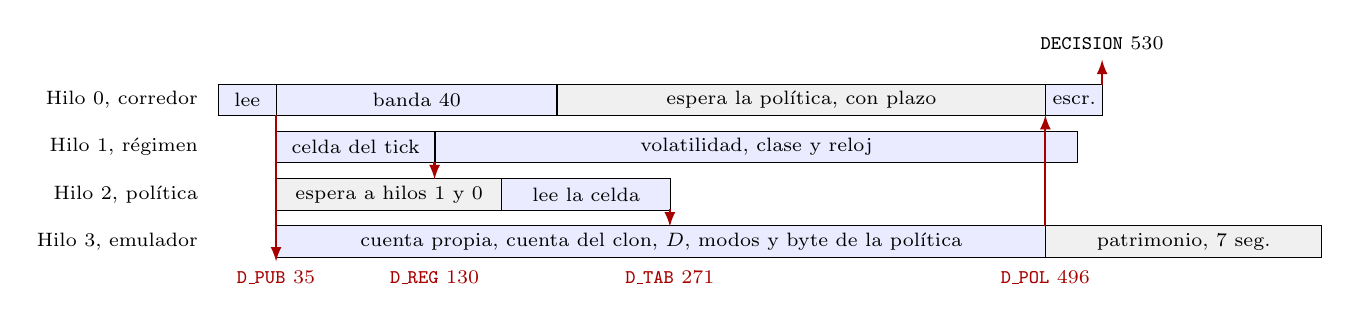
\begin{tikzpicture}[x=0.0212cm,y=0.60cm,font=\scriptsize,
    caja/.style={draw,fill=blue!8,minimum height=0.40cm,inner sep=1pt,anchor=west},
    espera/.style={draw,fill=gray!12,minimum height=0.40cm,inner sep=1pt,anchor=west},
    dato/.style={-latex,thick,red!65!black}]
  % Las posiciones horizontales son ciclos desde byte_done: los promedios medidos (macros de
  % generado/cifras_c1.tex) y, donde no hay un hito medido, una posición aproximada sin rótulo.
  \foreach \h/\n in {0/corredor,1/régimen,2/política,3/emulador}
    \node[anchor=east] at (-6,-\h) {Hilo \h, \n};
  % hilo 0
  \node[caja,minimum width=0.74cm] at (0,0) {lee};
  \node[caja,minimum width=3.56cm] at (\ctresHitoPub,0) {banda 40};
  \node[espera,minimum width=6.21cm] at (\ctresApagadaPeor,0) {espera la política, con plazo};
  \node[caja,minimum width=0.72cm] at (\ctresHitoPolProm,0) {escr.};
  % hilo 1
  \node[caja,minimum width=2.01cm] at (\ctresHitoPub,-1) {celda del tick};
  \node[caja,minimum width=8.16cm] at (\ctresHitoRegProm,-1) {volatilidad, clase y reloj};
  % hilo 2
  \node[espera,minimum width=2.86cm] at (\ctresHitoPub,-2) {espera a hilos 1 y 0};
  \node[caja,minimum width=2.14cm] at (170,-2) {lee la celda};
  % hilo 3
  \node[caja,minimum width=9.77cm] at (\ctresHitoPub,-3) {cuenta propia, cuenta del clon, $D$, modos y byte de la política};
  \node[espera,minimum width=3.5cm] at (\ctresHitoPolProm,-3) {patrimonio, 7 seg.};
  % datos publicados
  \draw[dato] (\ctresHitoPub,-0.32) -- (\ctresHitoPub,-3.42);
  \node[anchor=north,red!65!black] at (\ctresHitoPub,-3.42) {\texttt{D\_PUB} \ctresHitoPub};
  \draw[dato] (\ctresHitoRegProm,-1.32) -- (\ctresHitoRegProm,-1.68);
  \node[anchor=north,red!65!black] at (\ctresHitoRegProm,-3.42) {\texttt{D\_REG} \ctresHitoRegProm};
  \draw[dato] (\ctresHitoTabProm,-2.32) -- (\ctresHitoTabProm,-2.68);
  \node[anchor=north,red!65!black] at (\ctresHitoTabProm,-3.42) {\texttt{D\_TAB} \ctresHitoTabProm};
  \draw[dato] (\ctresHitoPolProm,-2.68) -- (\ctresHitoPolProm,-0.32);
  \node[anchor=north,red!65!black] at (\ctresHitoPolProm,-3.42) {\texttt{D\_POL} \ctresHitoPolProm};
  \draw[dato] (\ctresHitoDecProm,0.32) -- (\ctresHitoDecProm,0.85) node[anchor=south,black] {\texttt{DECISION} \ctresHitoDecProm};
\end{tikzpicture}
\caption{Flujo de un tick en R3. En rojo, lo que publica cada hilo y el ciclo promedio, contado desde \texttt{byte\_done}, en que lo hace.}\label{fig:tick}
\end{figure}

\begin{table}[!ht]\centering
\caption{Trabajo de cada hilo por tick y ciclo en que publica, ronda 3.}\label{tab:32h}
% Generado por tools/report.py (make report). No editar a mano.
\begin{tabular}{lrrrlrr}
\toprule
Hilo & IC mín. & IC prom. & IC máx. & Publica & Ciclo prom. & Ciclo máx. \\
\midrule
0, corredor & 100 & 132{,}7 & 196 & \texttt{D\_PUB} & 35{,}0 & 35 \\
1, régimen & 110 & 118{,}7 & 133 & \texttt{D\_REG} & 130{,}0 & 536 \\
2, política & 47 & 58{,}0 & 156 & \texttt{D\_TAB} & 270{,}9 & 665 \\
3, emulador & 129 & 156{,}5 & 218 & \texttt{D\_POL} & 496{,}4 & 742 \\
0, corredor &  &  &  & \texttt{DECISION} & 529{,}9 & 783 \\
\bottomrule
\end{tabular}
\par\smallskip{\footnotesize Ronda 3, serie de práctica, por el RTL. IC: instrucciones del hilo por tick fuera de su lazo de espera del precio (CPI 4 por hilo). Ciclo: ciclos desde \texttt{byte\_done} hasta que el hilo publica. Fuente: \texttt{docs/mediciones/c1/ticks.txt}.}

\end{table}

El hilo 0 no depende de que los otros estén vivos. Si la política del tick no llega dentro del plazo de 28 vueltas y la última que llegó es del tick anterior, sostiene esa orden si era de 63 y mantiene si era parcial; si es más vieja, pasa a modo seguro, que es la banda 40 sin política hasta el final de la ronda. Se probaron \ctresDegradacion{} fallas puestas a propósito, todas con la decisión esperada y a tiempo (\arch{docs/mediciones/c1/degradacion.txt}).

\subsection{Registros, memoria y operaciones que Espino no tiene}

Cada hilo usa su propio banco de 16 registros; el uso de cada uno está al comienzo de cada hilo en \arch{sw/c1.s}. Los datos están en \ctresPalabrasDatos{} palabras al final de la memoria de programa, desde \texttt{0x768}, y el programa ocupa \ctresPalabras{} de las 512 palabras, \ctresPalabrasCodigo{} de código. La única cantidad fraccionaria es la volatilidad: se guarda 64 veces la suma de las diferencias al cuadrado, y los cortes de las clases están en sesenta y cuatroavos.

Espino no tiene desplazamientos, multiplicación ni división, y el programa no usa la extensión de la ISA. Se resuelven así (\arch{docs/c1\_plan.md}, sección 3):
\begin{itemize}
  \item \textbf{Ejecutar una orden} sin dividir: con los múltiplos $p, 2p, \dots, 32p$, que cuestan 5 sumas por tick, se resta del saldo de mayor a menor mientras quede cantidad y alcance (rutina \texttt{ejecutar}, línea 541).
  \item \textbf{$D$ y el patrimonio}: producto por los 8 bits de $p$, duplicando y sumando (rutina \texttt{producto}, línea 620).
  \item \textbf{Media posición}: división con 9 restas y comparaciones (líneas 449 a 472).
  \item \textbf{Clase de volatilidad}: en vez de dividir por el tiempo, se compara la suma con siete sumas que crecen una constante por tick (línea 257).
  \item \textbf{Dos niveles por celda}: la palabra de 16 bits de la tabla guarda dos bytes, que se leen con \texttt{lbu}.
\end{itemize}

\subsection{Mismas decisiones que la referencia}

La referencia es \arch{ref/c1/c1.py}, que hace las mismas operaciones enteras en el mismo orden. El \texttt{sw/trade.s} que nombra el enunciado es la banda 40 de R0; el programa de R3 es \arch{sw/c1.s}, y \texttt{make c1-oficial} lo corre con el testbench del curso. Ese testbench, sin modificar, da 4/4 con un peor caso de \ctresOficialPeor{} ciclos y un \texttt{decisiones.csv} idéntico byte a byte al de la referencia; con la serie de práctica completa a los tres períodos también, con patrimonio \ctresPracticaW{} (\arch{docs/mediciones/c1/oficial.txt}). Por el RTL se compararon además los bytes y el estado interno, tick a tick, en Meta, Tesla, AMD y \ctresPuertaBVentanas{} ventanas reales, \ctresPuertaBTicks{} millones de ticks, y en \ctresSinteticasRtl{} series sintéticas, con cero diferencias (\arch{puerta\_b.txt} y \arch{series.txt}, en la misma carpeta).

Como C1 depende de llevar la cuenta de la maestra, esa cuenta se verificó aparte. La cuenta emulada coincide con la contabilidad del testbench oficial en \ctresContSeries{} series, con \ctresContParciales{} órdenes parciales y \ctresContDiferencias{} ticks de diferencia, y el RTL de R3 coincide con la maestra emulada en \ctresContRtl{} corridas (\arch{contabilidad.txt}, \arch{contabilidad\_rtl.txt}). En la placa, la autoprueba de R3 da la firma esperada a los tres ritmos (\arch{docs/bitacora/c1.md}, 21/11), y la integración local pasa \ctresIntegracionLocal{} pasos (\arch{docs/mediciones/ci\_local\_c1.txt}).

\subsection{Mediciones por tick}\label{sec:ticks}

La tabla~\ref{tab:32} da las instrucciones, los ciclos, el CPI y el tiempo desde que llega el precio hasta la escritura de \texttt{DECISION}. A 25\,MHz un ciclo dura 40\,ns, y el presupuesto de cada ronda es el período menos los 9,5\,$\mu$s de la transacción SPI: \ctresPresupuesto{} ciclos a 0,1\,ms.

\begin{table}[H]\centering
\caption{Instrucciones, ciclos, CPI y tiempo por tick de R3, promedio y peor caso, en las tres rondas.}\label{tab:32}
\tablaancha{generado/t32r3.tex}\par\smallskip
% Generado por tools/report_c1.py. No editar a mano.
{\footnotesize Respuesta: de \texttt{byte\_done} a la escritura en \texttt{DECISION}, serie de práctica completa a cada período, con el gemelo digital. El RTL da los mismos ciclos donde se midió: promedio y peor caso de la ronda 3 (\texttt{docs/mediciones/c1/ticks.txt}) y peor caso de las rondas 1 y 2 (\texttt{oficial.txt}). Presupuesto: ciclos del período menos la transacción SPI.\par}

\end{table}

En la ronda 3 la respuesta toma \ctresRespProm{} ciclos en promedio (\ctresRespPromUs\,$\mu$s) y \ctresRespPeor{} en el peor tick (\ctresRespPeorUs\,$\mu$s), el \ctresUsoPresupuesto\,\% del presupuesto. El CPI es 4 por hilo y 1 sumando los cuatro hilos, por construcción del barrel. A diferencia de la banda 40, el tiempo depende de los datos: la respuesta va de \ctresRespMin{} a \ctresRespPeor{} ciclos según el modo y la fase. El peor tick de todas las pruebas, con \ctresGemeloReales{} series reales y \ctresSinteticasGemelo{} sintéticas, es de \ctresPeorPuertas{} ciclos, y con un hilo colgado a propósito, de \ctresPeorColgado: siempre menos de la mitad del presupuesto, \ctresLimiteGrupo{} ciclos, que es el límite que se fijó el grupo (\arch{docs/puertas.md}).

% ==============================================================================
\section{Co-diseño hardware/software (3.3)}

\subsection{La escalera de R0 a R3}

Además del Espino base se construyeron, verificaron y midieron cinco alternativas de hardware (tabla~\ref{tab:escalera}):
\begin{itemize}
  \item \textbf{Segmentado}: pipeline de 3 etapas que lee la memoria de instrucciones en el flanco de bajada. Ataca el CPI.
  \item \textbf{Barrel}: cuatro hilos que rotan por un pipeline de 4 etapas, sin adelantamiento ni burbujas. Cada hilo va más lento, con CPI 4, pero el procesador completa una instrucción por ciclo.
  \item \textbf{R1 y R2}: el barrel con los umbrales en una tabla en BRAM, que se cambia sin sintetizar de nuevo, y en R2 un vigilante que reconfigura la FPGA con R0 si el hilo 0 deja de escribir \texttt{DECISION}.
  \item \textbf{R3}: R2 con la tabla de 512 palabras, que es el único hardware que C1 agrega.
  \item \textbf{Extensión de la ISA} en custom-0, \texttt{emad} y \texttt{devk}: sobre el barrel baja el kernel de la regla anterior, de media exponencial, de \pSieteAmdahlCiclosPredKernelBarrel{} a \pSieteAmdahlCiclosPredKernelXdSobreBarrel{} ciclos, con \pSieteCeldasBarrelXd{} celdas contra \pSieteCeldasBarrel. El hardware de R1 a R3 la conserva, pero ni la banda 40 ni C1 llevan una media y no la usan (\arch{docs/extension\_isa.md}).
\end{itemize}

\begin{table}[H]\centering
\caption{La escalera de co-diseño: recursos, respuesta, CPI y desempeño logrado de cada peldaño.}\label{tab:escalera}
\tablaancha{generado/t33r3.tex}\par\smallskip
% Generado por tools/report_c1.py. No editar a mano.
{\footnotesize R0 a R2 corren la banda 40 y R3 corre C1. Recursos: 10 semillas de nextpnr a 25 MHz, todas cierran; $f_{\max}$ es la mínima. Respuesta en ciclos, práctica a 0,1 ms; \% presup.: peor caso sobre 2\,262 ciclos. CPI del kernel (4 por hilo en el barrel). MOPS = operaciones útiles $\times$ 25 MHz / ciclos del kernel. Fuentes: \texttt{docs/mediciones/p7/cotas/variantes.txt}, \texttt{docs/mediciones/c1/timing.txt} y \texttt{ops\_roofline.txt}. $^*$R3 usa otra definición de operación útil, el conteo por clase de instrucción: en esa escala la banda 40 tiene 21 operaciones y no 11, R0 logra 10{,}50 MOPS y R2 3{,}12.\par}

\end{table}

Del Espino base al segmentado la respuesta baja a la mitad con menos celdas, y del segmentado al barrel sube casi cuatro veces, porque un programa de un solo hilo usa uno de cada cuatro ciclos. R2 es el peldaño de menor desempeño logrado, \ctresRdosMops{} MOPS contra \ctresRceroMops{} de R0, porque tres de sus cuatro hilos esperan. R3 rompe la tendencia en los dos sentidos: es el que más tarda en responder, \ctresRespPeor{} ciclos contra \ctresRdosRespPeor{} de R2, y el único que ocupa los cuatro hilos. La fila de R2 es la síntesis de su bitstream; sintetizado con su programa actual ocupa \ctresCeldasRdosMismaSintesis{} celdas (\arch{docs/mediciones/fondo/r2/timing.txt}), así que la tabla de 512 palabras cuesta \ctresCeldasSobreRdos{} celdas y un BRAM.

\textbf{Operación útil.} En la banda 40 son las 11 operaciones de la regla por tick, contadas a mano: 4 comparaciones con los umbrales, 2 que recuerdan los extremos vistos, 1 que los reúne y 4 que arman comprar y vender (\arch{tools/p7/cotas.py}). En C1 la cantidad depende de los datos, y se cuentan sobre el perfil las instrucciones aritméticas, lógicas y de comparación de los cuatro hilos; no cuentan loads, stores, saltos, cargas de constantes, esperas ni telemetría. Son \ctresOps{} por tick y \ctresMops{} MOPS (\arch{docs/mediciones/c1/ops\_roofline.txt}). Ese conteo es más amplio que el manual: aplicado a la banda 40 da \ctresOpsBandaPorClase{} operaciones, \ctresMopsRceroPorClase{} MOPS en R0 y \ctresMopsRdosPorClase{} en R2. En la misma escala, R3 logra \ctresMopsSobreRdos{} veces el trabajo útil por segundo de R2 con el mismo procesador, y queda debajo de R0.

\subsection{En qué se gastan los ciclos y qué predice Amdahl}

Entre variantes de procesador, Amdahl generalizado se comprobó midiendo (tabla~\ref{tab:amdahl}): las fracciones $f_i$ salen del perfil de R0 y los factores $F_i$, de aplicar a cada fase el costo por clase de instrucción de la variante nueva. Al pasar al barrel el speedup predicho del kernel es \ctresAmdahlBarrelPred{} y el medido \ctresAmdahlBarrelMed. En el segmentado, con el CPI que estimó la clase 7 la predicción del kernel queda \pCotasAmdahlErrKernelSegClase\,\% bajo lo medido: la clase suponía 3 ciclos por salto tomado y se miden 2. Lo que peor se predice es la respuesta, por la fase en que cae el precio respecto del sondeo.

\begin{table}[H]\centering
\caption{Speedup predicho por Amdahl contra el medido, con la banda 40.}\label{tab:amdahl}
% Generado por tools/report.py (make report). No editar a mano.
\begin{tabular}{llrrr}
\toprule
Ventana & Cambio & $S$ predicho & $S$ medido & Ciclos pred. / med. \\
\midrule
Respuesta & R0 $\to$ segmentado, CPI de la clase 7 & 1{,}815 & 2{,}018 & 31{,}12 / 28{,}00 \\
Respuesta & R0 $\to$ segmentado, costo medido & 1{,}887 & 2{,}018 & 29{,}94 / 28{,}00 \\
Respuesta & R0 $\to$ barrel, un hilo & 0{,}532 & 0{,}528 & 106{,}25 / 107{,}00 \\
Kernel & R0 $\to$ segmentado, CPI de la clase 7 & 1{,}852 & 1{,}923 & 27{,}00 / 26{,}00 \\
Kernel & R0 $\to$ segmentado, costo medido & 1{,}923 & 1{,}923 & 26{,}00 / 26{,}00 \\
Kernel & R0 $\to$ barrel, un hilo & 0{,}521 & 0{,}521 & 96{,}00 / 96{,}00 \\
\bottomrule
\end{tabular}
\par\smallskip{\footnotesize Amdahl generalizado, $S = 1 / \sum_i (f_i / F_i)$, con las fracciones del perfil de R0. Fuente: \texttt{docs/mediciones/p7/cotas/amdahl.txt}.}

\end{table}

En R3 el perfil por hilo y por rutina (\arch{docs/mediciones/c1/perfil\_hilos.txt}) muestra que la respuesta la cierra el hilo 3. Publica la política a los \ctresHitoPolProm{} ciclos en promedio, y el hilo 0, que terminó la banda 40 antes y esperó \ctresEsperaHiloCero{} ciclos, escribe \texttt{DECISION} a los \ctresHitoDecProm. Lo que más pesa en el hilo 3 es la rutina \texttt{ejecutar}, las dos cuentas: \ctresEjecutarIc{} instrucciones y \ctresEjecutarCiclos{} ciclos por tick, el \ctresAmdahlF\,\% de la respuesta. Con $S = 1/((1-f) + f/F)$, aun con una contabilidad en hardware de costo cero el speedup de la respuesta no pasa de \ctresAmdahlSmax, y la respuesta bajaría a unos \ctresAmdahlRespMin{} ciclos. Esa variante no se construyó, así que para R3 hay predicción y no speedup medido. Tampoco se justifica: la respuesta ya ocupa el \ctresUsoPresupuesto\,\% del presupuesto, y responder antes no cambia ninguna decisión.

\subsection{Roofline}

En el roofline (figura~\ref{fig:roofline}) el ancho de banda de Pochoco es $B_s = 4$~B por ciclo a 25\,MHz, \pSieteBs\,MB/s. Cada variante tiene su techo $P_{peak} = f \times \text{instrucciones por ciclo} \times \text{operaciones por instrucción}$: 12,5 MOPS el Espino base, 25 el segmentado, 6,25 el barrel con un hilo útil y 25 el barrel con sus cuatro hilos. Todos los kernels quedan a la derecha del quiebre de su variante, limitados por cómputo y no por memoria, y ninguno llega a su techo porque leer, escribir, saltar y esperar no son operaciones útiles. R3 queda en \ctresIntensidad\,Op/B, con menos operaciones por byte que la banda 40 de R0 porque los hilos se pasan los datos por memoria.

\begin{figure}[H]\centering
\resizebox{0.74\linewidth}{!}{% roofline_r3.tex: generado por tools/report_c1.py desde docs/mediciones/p7/cotas/roofline.tex y c1/ops_roofline.txt.
% Ejes en log10: x de 0,01 a 100 Op/B, y de 0,1 a 100 MOPS.
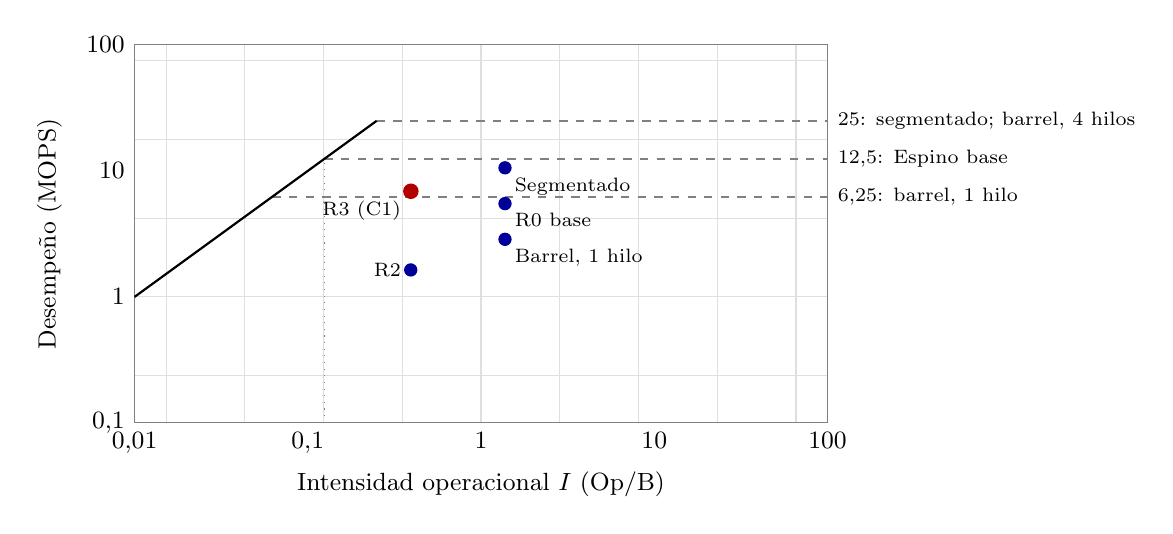
\begin{tikzpicture}[x=2.2cm,y=1.6cm,font=\small]
  \draw[gray!25] (-2,-1) grid (2,2);
  \draw[gray] (-2,-1) rectangle (2,2);
  \node[below] at (-2,-1) {$0{,}01$};
  \node[below] at (-1,-1) {$0{,}1$};
  \node[below] at (0,-1) {$1$};
  \node[below] at (1,-1) {$10$};
  \node[below] at (2,-1) {$100$};
  \node[left] at (-2,-1) {$0{,}1$};
  \node[left] at (-2,0) {$1$};
  \node[left] at (-2,1) {$10$};
  \node[left] at (-2,2) {$100$};
  \node[below=5mm] at (0.0,-1) {Intensidad operacional $I$ (Op/B)};
  \node[rotate=90,above=8mm] at (-2,0.5) {Desempeño (MOPS)};
  \draw[gray,dashed,thick] (-1.2041,0.7959) -- (2,0.7959) node[right,black,font=\scriptsize] {6{,}25: barrel{,} 1 hilo};
  \draw[gray,dashed,thick] (-0.9031,1.0969) -- (2,1.0969) node[right,black,font=\scriptsize] {12{,}5: Espino base};
  \draw[gray,dashed,thick] (-0.6021,1.3979) -- (2,1.3979) node[right,black,font=\scriptsize] {25: segmentado; barrel{,} 4 hilos};
  \draw[black,thick] (-2,0.0000) -- (-0.6021,1.3979);
  \draw[gray,dotted] (-0.9031,-1) -- (-0.9031,1.0969);
  \filldraw[blue!60!black] (0.1383,0.7404) circle (2.2pt) node[below right,font=\scriptsize,black] {R0 base};
  \filldraw[blue!60!black] (0.1383,1.0244) circle (2.2pt) node[below right,font=\scriptsize,black] {Segmentado};
  \filldraw[blue!60!black] (0.1383,0.4571) circle (2.2pt) node[below right,font=\scriptsize,black] {Barrel, 1 hilo};
  \filldraw[blue!60!black] (-0.4058,0.2140) circle (2.2pt) node[left,font=\scriptsize,black] {R2};
  \filldraw[red!70!black] (-0.4049,0.8385) circle (2.6pt) node[below left,font=\scriptsize,black] {R3 (C1)};
\end{tikzpicture}
}
\caption{Roofline de Espino con los techos de cada variante. En azul, el kernel de la banda 40 en cada peldaño; en rojo, el de C1 en R3, con el conteo por clase de instrucción.}\label{fig:roofline}
\end{figure}

\subsection{PLL}

El encapsulado VQ100 de la Go Board no tiene PLL: nextpnr termina con \emph{PLL couldn't be placed anywhere, no suitable BEL found} (\arch{docs/mediciones/p7/pll.txt}). Un duplicador de reloj por lógica cierra timing en \pSieteDobleSemillas{} de \pSieteDobleSemillasTotal{} semillas con el segmentado y en ninguna con el Espino base (\arch{docs/mediciones/p7/negativos.txt}). No se subió la frecuencia, y el presupuesto de cada ronda es el de 25\,MHz.

\subsection{Variante final: por qué compite la más lenta}

Compite R3, que es la variante que más tarda en responder. La velocidad no entra en el patrimonio: todas las variantes escriben \texttt{DECISION} antes del tick siguiente, y la maestra ejecuta la orden al mismo precio haya llegado en \ctresSegRespPeor{} ciclos o en \ctresRespPeor. Lo que el período más corto deja son \ctresPresupuesto{} ciclos por tick, y la banda 40 usa \ctresRdosRespPeor{} en R2. R3 gasta los que sobran en lo que sí cambia el resultado: emular al rival con dos cuentas exactas en un hilo, medir la volatilidad en otro y consultar la política del modelo en la tabla. Ese trabajo son \ctresTrabajoSerie{} instrucciones por tick sin contar esperas. En un solo hilo del barrel serían unos \ctresTrabajoSerieCiclos{} ciclos en promedio, una estimación porque ese programa no se escribió; repartido en los cuatro hilos, la respuesta promedio es de \ctresRespProm{} (\arch{docs/mediciones/c1/ops\_roofline.txt}).

El costo en hardware es de \ctresCeldas{} de 1\,280 celdas y \ctresBram{} de 16 BRAM, con \ctresFmin\,MHz de frecuencia mínima en \ctresSemillas{} semillas (\arch{docs/mediciones/c1/timing.txt}). El riesgo queda acotado por diseño: con la política apagada o con un hilo colgado R3 decide la banda 40, y si el hilo 0 deja de escribir, el vigilante carga R0, el Espino base con la banda 40. La elección no es la variante más rápida ni la de más MOPS, sino la que convierte los ciclos libres del tick en ganar sola más veces: \ctresExamenGana\,\% de los torneos contra \ctresExamenGanaBanda\,\% en el examen.
